\section{Background}
\label{sec:background}

\subsection{Reinforcement learning}

This entire section is descriptions of key concepts from a book on
Reinforcement Learning by Sutton and Barto \cite{sutton1998reinforcement}. If
no other reference is explicitly mentioned, statements are taken from this
book.

\subsubsection{The three tiers of machine learning}

In reinforcement learning (RL) an agent interacts with an environment and tries
to maximize how much \textit{reward} it can receive from the environment. To
maximize the reward in the long run might require short-time losses, making the
problem more complex than just maximizing for one step at a time. To find a
good strategy, commonly referred to as a \textit{policy}, the agent uses its
experience to make better decisions, this is referred to as
\textit{exploitation}. But, it must also find a balance between exploitation
and to also try out new things, i.e. \textit{exploration}. These features are
specific for RL and therefore distinguishes it from supervised and unsupervised
learning making it the third tier of machine learning.

\subsubsection{Main elements of RL}

Let $S_t$ be the state at time $t$, $R_t$ be the reward at time $t$, and $A_t$
the action at time $t$. The interaction between an agent and its environment in
RL is depicted in figure \ref{fig:rl_flowchart}. At time step $t$, the agent
reads the environment state and takes an action. The environment changes, maybe
stochastically, by responding with a new state $S_{t+1}$ and a reward $R_{t+1}$
at time $t+1$. 

\begin{figure}[h]
    \centering
    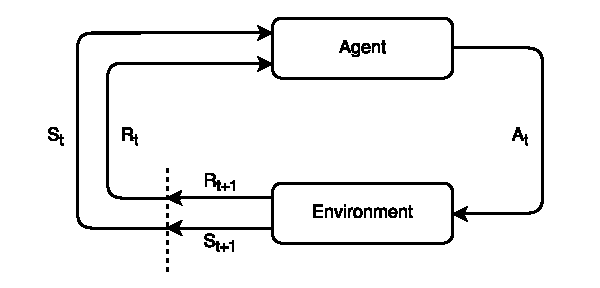
\includegraphics[]{res/agent_environment_interaction.pdf}

    \caption{Agent and environment interaction in RL. $S_t$, $R_t$, and $A_t$
             is the state, reward, and action at time $t$ \cite{sutton1998reinforcement}.}

    \label{fig:rl_flowchart}
\end{figure}

The quantity to maximize is often not the immediate rewards, but rather the
long term accumulated rewards. Let us call this quantity $G_t$, or
\textit{return}, for an agent at time $t$ up to some time $K$:

\begin{equation}
    G_t = \sum_{k=0}^K \gamma^k R_{t+k+1}
\end{equation}

Some problems imply that $K$ can go to infinity, and for $\gamma = 1$, $G_t$
can theoretically take infinite values. It is obviously problematic to maximize
something infinite and that is the reason for the $\gamma \in \left[0,
1\right]$ factor above that alleviates this problem if $\gamma < 1$ (proof
omitted). For lower values of $\gamma$ the agent tries to maximize short term
rewards, and for larger values long-term rewards. 

A policy is a function from the state of the environment to probabilities over
actions, i.e. the function that chooses what to do in any situation. Since a
reward is only short-term, a \textit{value function} tries to estimate the
total amount of reward that will be given in the long run for being in some
state and following some policy. To enable planning of actions in the
environment, RL algorithms sometimes use a \textit{model} in order to
explicitly build up an understanding of the environment. This is usually
referred to as \textit{model-based} RL in contrast to \textit{model-free}.

\subsubsection{Finite Markov Decision Processes}

In a RL scenario where the environment has a finite number of states, there is
a finite number of actions, and the Markov property holds is called a
\textit{finite Markov Decision Process} (finite MDP). The dynamics of a finite
MDP are completely specified by the probability distribution:

\begin{equation}
    p(s', r|s, a) = P(S_{t+1} = s', R_{t+1} = r | S_t = s, A_t = a)
\end{equation}

Important functions and terminology that is used throughout RL includes the
\textit{state-value function} (abbreviated as value function) and the
\textit{action-value function}. The state-value function with respect to some
policy informally gives how good a state is to be in given that
the policy is followed thereafter:

\begin{equation}
    v_\pi(s) = \mathbb{E}_\pi\left[G_t|S_t=s\right] = \mathbb{E}_\pi\left[\sum_{k=0}^\infty \gamma^k R_{t+k+1}|S_t=s\right]
\end{equation}

To compare the value of different actions in some state, given that you thereafter follow some policy $\pi$,
is given by the action-value function:

\begin{equation}
    q_\pi(s, a) = \mathbb{E}_\pi\left[G_t|S_t=s,A_t=a\right] = \mathbb{E}_\pi\left[\sum_{k=0}^\infty \gamma^k R_{t+k+1}|S_t=s,A_t=a\right]
\end{equation}

According to RL theory there is always an optimal policy
\cite{sniedovich1986new}, i. e. that gives the highest possible expected return
given any state. This is often denoted with $*$ and has the corresponding value
and action-value functions $v_*(s)$ and $q_*(s, a)$. Given the optimal value or
action-value function, it is (depending on the problem) easy to infer the
optimal policy, therefore a common approach is to first approximate either of
these functions.

\subsubsection{Policy and value iteration}

One exact method to find the optimal policy, at least in the limit, is called
\textit{policy iteration}. This builds on two alternating steps, the first
called \textit{iterative policy evaluation}. This estimates a value function
given some policy and starts from a random value function $v_0$, except for any
terminal state $s_K$ for which are assigned $v_0(s_K) = 0$. By $v_k$ is meant
the value function estimate at iteration $k$. Then we iteratively update new
value functions for each step:

\begin{align*}
    v_{k+1}(s) &= \mathbb{E}\left[R_{t+1} + \gamma v_{k}(S_{t+1}) | S_t=s \right] \\
               &= \sum_a \pi (a|s) \sum p(s', r|s, a) \left[r + \gamma v_k(s')\right]
\end{align*}

As can be seen, the dynamics $p(s', r|s, a)$ needs to be known, which of course
is not always the case. The next step is called \textit{policy improvement} and for this
we first need to calculate the action-state function given the current policy
$\pi$:

\begin{align*}
    q_\pi(s, a) &= \mathbb{E}\left[R_{t+1} + \gamma v_\pi(S_{t+1}) | S_t=s, A_t = a \right] \\
                &= \sum_{s', r} p(s', r|s, a) \left[r + \gamma v_\pi(s')\right]
\end{align*}

Given this, an improved policy $\pi'$ is attained by:

\begin{equation}
    \pi'(s) = \text{arg}\max_a q_\pi(s, a)
\end{equation}

Iteratively performing these two steps will eventually converge to the optimal
policy \cite{puterman1979convergence}. There is an alternative way that is done by only approximating the
value function, called \textit{value iteration}:

\begin{align*}
    v_{k+1}(s) &= \max_a \mathbb{E}\left[R_{t+1} + \gamma v_k(S_{t+1}) | S_t=s, A_t = a \right] \\
             &= \max_a \sum_{s', r} p(s', r|s, a) \left[r + \gamma v_k(s')\right]
\end{align*}

After convergence to some value function $v$, the optimal policy is found by:

\begin{equation}
    \pi'(s) = \text{arg}\max_a \sum_{s', r} p(s', r|s, a) \left[r + \gamma v(s')\right]
\end{equation}

\subsubsection{Monte Carlo methods and Temporal-Difference learning}

Policy and value iteration are exploring the entire state-action space and
finds an optimal policy if the dynamics of the environment are known. Sometimes
we are dealing with samples from interacting with a system, and where we do not
know the dynamics. For these cases, we can instead estimate the action-value
function given a policy. This can be done by \textit{Monte Carlo methods} which
in its simplest form is averaging of returns for samples that we have attained.
The other method is \textit{Temporal-difference methods} which estimates an error
for each observed reward and updates the action-value function with this. To be
more precise, one famous example of a time difference method is
\textit{Q-learning} and the updates are done according to:

\begin{equation}
    Q(S_t, A_t) \leftarrow Q(S_t, A_t) + \alpha \left[ R_{t+1} + \gamma \max_a Q(S_{t+1}, a) - Q(S_t, A_t) \right]
\end{equation}

Q-learning is an example of an \textit{off-policy} method. This means that you
can use a second, or derived, policy for exploration, but the algorithm still
finds the optimal policy. The other family of methods is called
\textit{on-policy} methods and are characterized by that the expectation being
maximized is with respect to the exploring policy. In contrast to this the
expectation in the off-policy case is only dependent on the environment.

\subsection{Neural networks}

\subsubsection{Basic idea}

The simplest neural network could be considered to be a linear transformation
of some data points $X$:

\begin{equation}
    X_1 = WX + B
\end{equation}

Since for some column in $X$, all its values influence all the values in the
same column in $X_1$, the \textit{input layer} $X$ and \textit{layer} $X_1$ are
said to be \textit{fully connected}. The convention of describing neural
networks with layers comes from the inspiration of physical neurons arranged in
layers although the description is not as apparent when describing the networks
in this fashion. The above transformation is obviously restricted to learning
linear transformations, so to learn non-linear functions, a
non-linear \textit{activation-function} is added:

\begin{equation}
    X_1 = f(WX + B)
\end{equation}

To learn more complex functions, transformations can be recursively stacked:

\begin{align}
    X_2 &= f(W_1X_1 + B_1)\\
    ...\\
    Y_{k+1} &= f(W_kX_k + B_k)
\end{align}

A loss function is a function $\ell : f, \mathbb{R}^d \longmapsto \mathbb{R}$,
where $f$ is the neural network and $\mathbb{R}^d$ is some data. Usually, the
data are inputs to the network, often along with corresponding target values.
This specifies the error, and implicitly the wanted behavior of the network. By
all parts being differentiable we can specify the loss function and calculate
its derivatives with respect to all the parameters $W, W_1,...$ and $B, B_1,
...$.  Using this we can then minimize the loss using gradient descent. A
common and effective way to do this is called \textit{back-propagation}
\cite{williams1986learning}.  The first layer $X$ is commonly referred to as
the input layer and the last layer as the output layer. The intermediate values are
referred to as hidden layers.

\subsubsection{Common activation functions}

Two common activation functions include \textit{tanh} and \textit{Rectified
Linear Unit} (ReLU) \cite{jarrett2009best} shown in figure \ref{fig:tanh_relu}. The tanh function is defined as:

\begin{equation}
    \tanh(x) = \frac{2}{1+e^{-x}} - 1
\end{equation}

The ReLU is defined as:

\begin{equation}
    \text{relu}(x) = \max (0, x)
\end{equation}

Another addition to the family of activation functions is the
\textit{exponential linear unit} (ELU) \cite{clevert2015fast} which has the
benefit of propagating the gradient also for negative input values since the
limit for large negative input values is $-1$ rather than $0$ as for the ReLU.
This was shown to speed up training and lowering classification test errors.
The ELU is defined as (with $\alpha$ usually being set to $1.0$):

\begin{equation}
    f(\alpha, x) =
    \begin{cases}
        \alpha (e^{x} - 1) & \text{if } x < 0 \\
        x & \text{if } x \geq 0
    \end{cases}
\end{equation}

For classification networks, a common function to have in the output layer is
the softmax function shown in figure \ref{fig:softmax}. A property of the
softmax is that all values will be output in the range $[0, 1]$ and sum to one,
making it conveniently interpreted as probabilities of different classes or
categories. The mathematical definition is for a set $x_1, ..., x_K$:

\begin{equation}
    \text{softmax}(x_k|x_1, ..., x_K) = \frac{e^{x_k}}{\sum_{i=1}^K e^{x_i}}
\end{equation}

\begin{figure}[h]
    \centering
    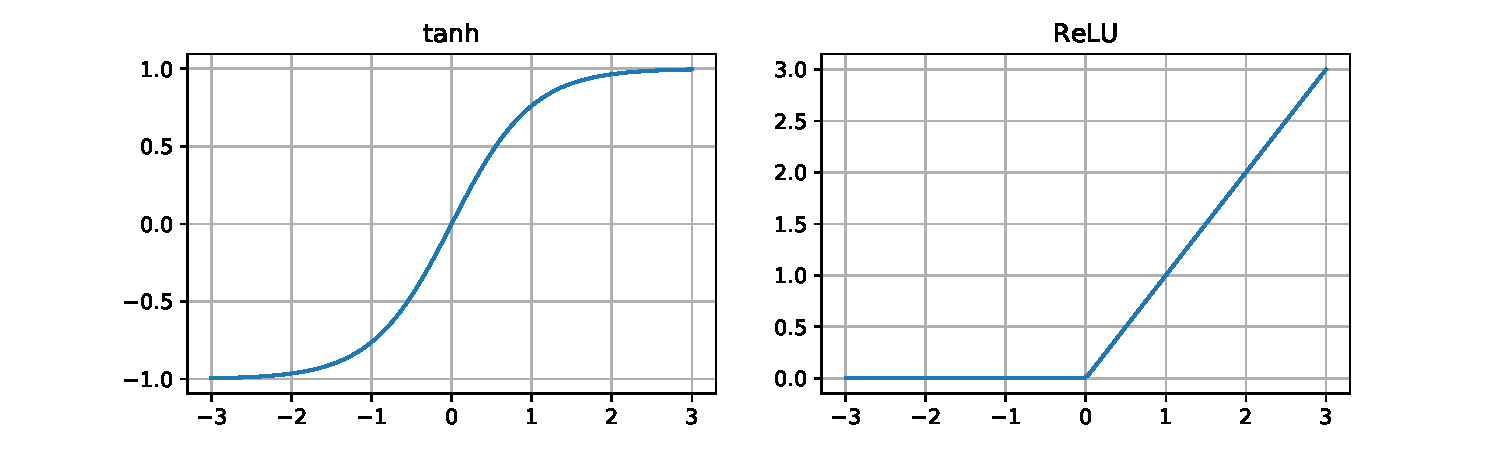
\includegraphics[width=0.8\textwidth]{res/relu_tanh.pdf}

    \caption{Common activation functions for neural networks.}

    \label{fig:tanh_relu}
\end{figure}

\begin{figure}[h]
    \centering
    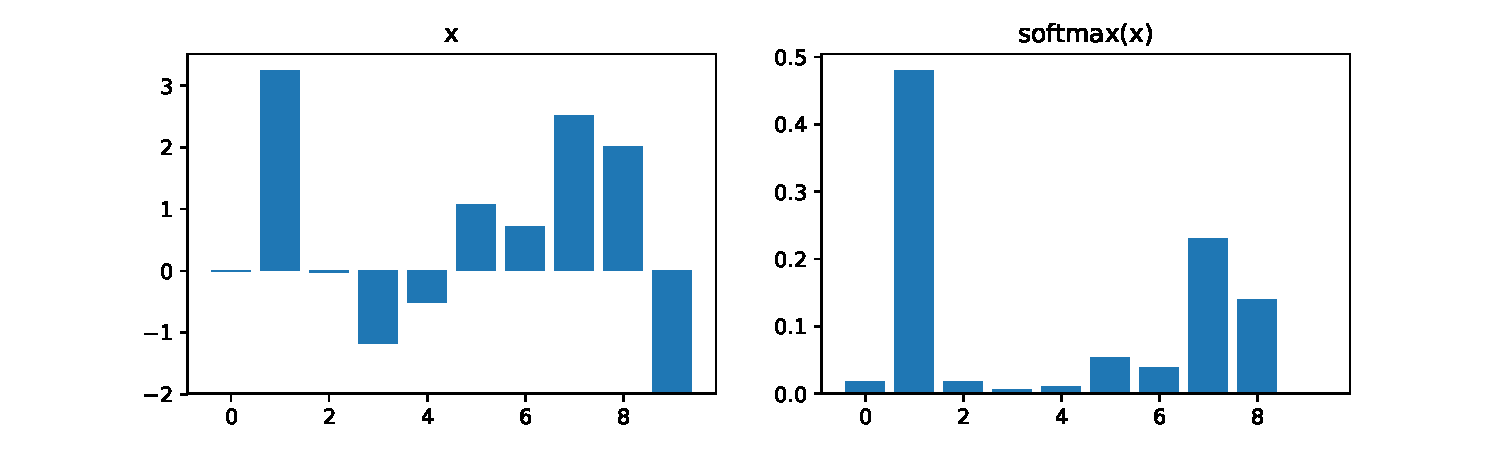
\includegraphics[width=0.8\textwidth]{res/softmax.pdf}

    \caption{Softmax function commonly used to convert a set of numbers $\in
    \mathbb{R}$ to probabilities of a discrete set of categories.}

    \label{fig:softmax}
\end{figure}

\subsubsection{Weight sharing}

In order to construct effective models with less number of parameters the fact
is used that some features are invariant of where in the data they are, e.g.
the pattern $1, 2, 3, 4$ in the beginning, middle, or the end of the data. To
this end, convolutions are used (where $*$ is the convolution operator):

\begin{equation}
    y = w * x + b
\end{equation}

These kind of networks are usually referred to as \textit{convolutional neural
networks} (CNN) \cite{lecun1989backpropagation}. The notation becomes a bit
more tricky here since the convolutions are commonly done in two dimensions
with 3-dimensional kernels ($w$). These are commonly used in neural networks
for images. It is common to use an other form of layer in conjunction with
convolutional layers called \textit{pooling} layers. These are used to reduce
the dimensionality from one layer to another and are very similar to
convolutions, but instead of kernels with varying weights, a max operation
\cite{huang2007unsupervised} or average operation \cite{lecun1998gradient} is
applied (average pooling is a kernel with all weights being equal).

\subsubsection{Optimizers}

A method commonly used for optimizing neural networks is called Adam
\cite{kingma2014adam}. Updates to parameters of the function with loss function
$f(\theta)$ are done by first and second order estimates of the gradients $g_t
= \nabla_{\theta_t} f(\theta_{t-1})$. The current timestep is annotated $t$ and
starts with $t = 1$, this is used to bias-correct the first and second order
estimates:

\begin{equation}
    m_t = \beta_1 m_{t-1} + (1 - \beta_1) g_t
\end{equation}

\begin{equation}
    v_t = \beta_2 v_{t-1} + (1 - \beta_2) g_t^2
\end{equation}

\begin{equation}
    \mathbb{E}\left[g \right] \approx \hat{m}_t = \frac{m_t}{1- \beta_1^t}
\end{equation}

\begin{equation}
    \mathbb{E}\left[g^2 \right] \approx \hat{v}_t = \frac{v_t}{1- \beta_2^t}
\end{equation}

Here $\beta_1, \beta_2 \in [0, 1)$ are hyperparameters. The updates are done
with stepsize $\alpha$ according to ($\epsilon >0$ to ensure no division by zero):

\begin{equation}
    \theta_t = \theta_{t-1} - \alpha \frac{\hat{m}_t}{\sqrt{\hat{v}_t - \epsilon}}
\end{equation}

Adam can be seen as a generalization of RMSProp where $\beta_1 = 0$
\cite{tieleman2012lecture} which implies that only a running second order
estimate is used. This has been successfully used for training of on-policy
algorithms \cite{mnih2016asynchronous} where gradients from previous policies
included in the running mean might not be suitable for current policy updates.
Earlier commonly used methods include Adadelta \cite{zeiler2012adadelta},
Adagrad \cite{duchi2011adaptive}, and momentum \cite{qian1999momentum}.


\subsubsection{Avoiding overfitted networks}

A classical approach to regularize neural networks is adding a scaled L2-norm
of the parameters to the loss. Another way shown to be effective, both for
fully connected and convolutional neural networks, is called dropout
\cite{srivastava2014dropout}. During training time, units are with probability
$p$ set to zero and non-zeroed outputs are scaled by $1/p$. Effectively, this
means inference during training time is done using random subgraphs of the
neural network, and inference during test time is done by average voting from a
collection of those subgraphs. To alleviate the problem of overfitting when
using images, it is common to use data augmentation, i. e. applying random
scaling, translations, noise etc. to the images (e.g.
\cite{ciregan2012multi,simard2003best,krizhevsky2012imagenet}). Another
approach is to synthetically generate a larger image database by overlaying
parts of the images with patches of other objects \cite{ghadirzadeh2017deep}.

\subsubsection{Batch normalization}

As the weights in one layer changes during training, the following layers have
to adapt to this change. In fact, later layers constantly have to adopt to
changes in any of the previous layers during training, something called
\textit{internal covariance shift}. It was shown that this problem can be
solved by adding intermediate normalization layers, called \textit{batch
normalization} \cite{ioffe2015batch}. These layers whiten the activations of
the previous layer, i. e. element-wise subtraction of the mini-batch mean and
divide by the square root of the variance. Since the statistics are calculated
per mini-batch, they argue that this acts as a regularizer, and they
empirically show that dropout in some cases are no longer needed. They argue
that this is due to that the representation of one sample will shift
differently depending of the other samples in the mini-batch. For some cases,
whitening the outputs of the previous layer decreases what the next layer can
represent, e. g. not saturating the sigmoid function in the subsequent layer.
To alleviate this problem, the authors propose learnable parameters that ensure
that the normalization layer, if needed, can represent the identity function.
During inference, normalization is done on population estimates of the mean and
variance. These population estimates are inferred using running mean and
variance estimates attained during training. Using batch normalization showed
to decrease the number of training steps by a factor of 14 for some cases, and
improving the test errors of previous state-of-the-art networks.

\subsection{Problem statement}

Manipulation tasks that seem trivial to a human can be hard to learn for
robots, especially from scratch without initial human demonstration, due to
high sample complexity. Recent research suggests ways to do this but are often
based on that you know the poses of the objects and the end-effector. For some
scenarios these are non-trivial to find out. Using a camera for pose detection
has shown promising results but still assumes known camera offset or a fixed
position of the camera.

\subsection{Research question}

How can deep and distributed reinforcement learning be used for learning and
performing dynamic manipulation tasks with unknown poses.
